\begin{figure}[ht]
  \centering

  \caption{Github project exhibits} \label{fig:dask-screenshots}

  \medskip
  \begin{subfigure}[b]{0.9\textwidth}
    \centering
    \caption{GitHub project homepage for \texttt{dask/dask}.}\label{fig:dask-home}
    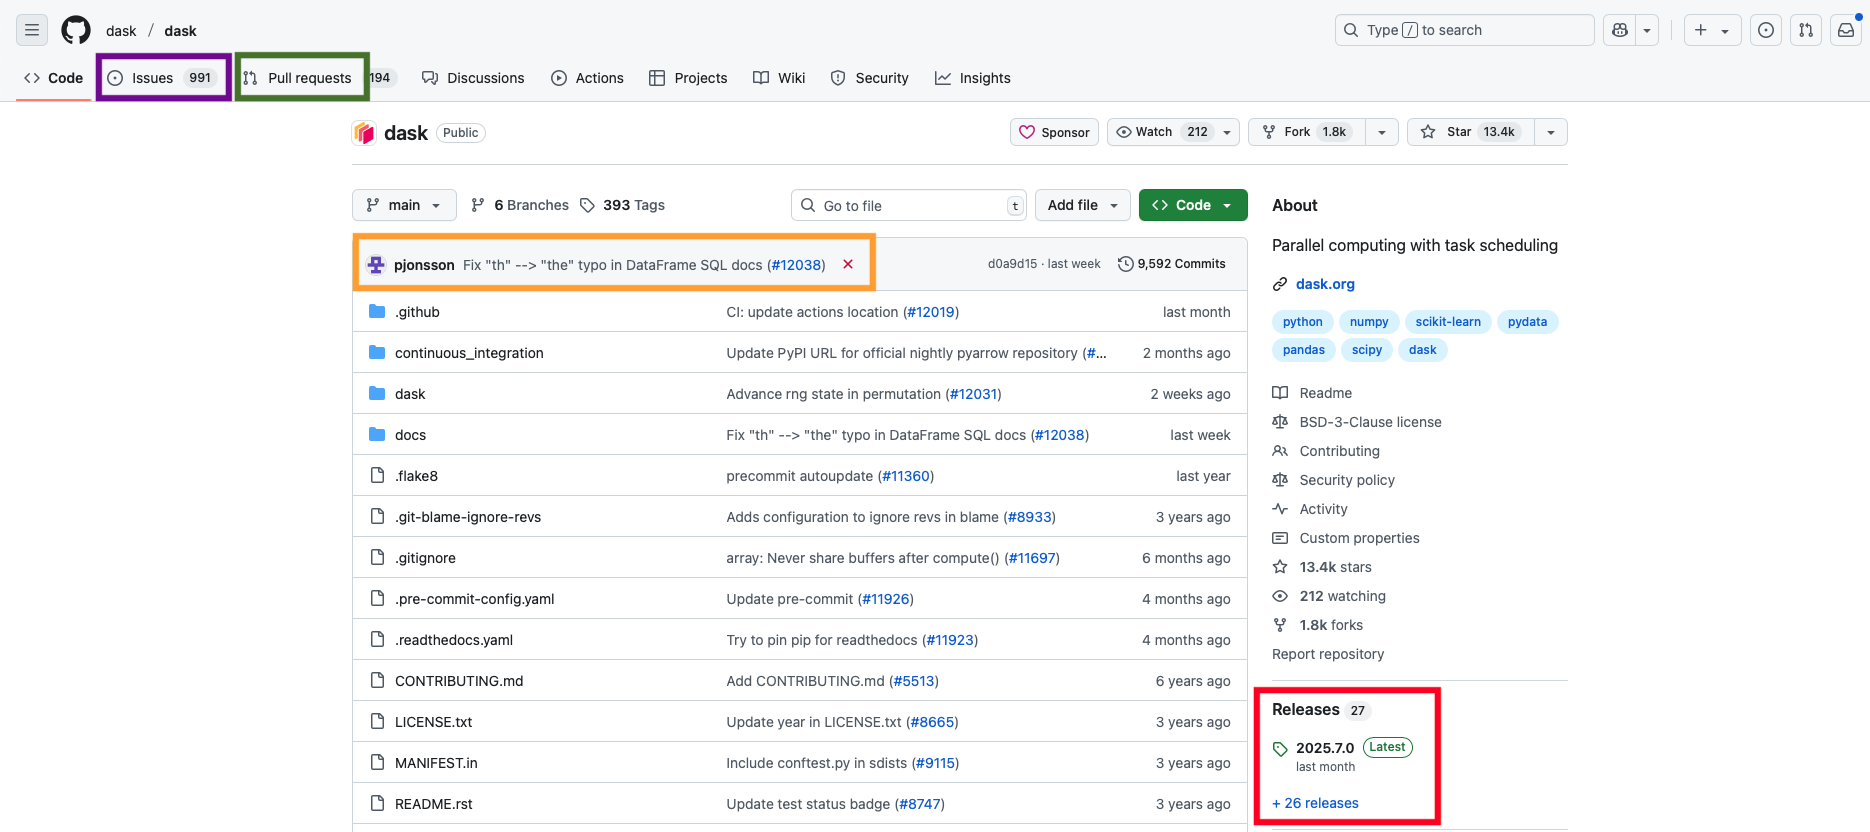
\includegraphics[width=\textwidth]{temp/dask_explainers/dask_homepage.png}
  \end{subfigure}

  \medskip

  \begin{subfigure}[b]{0.9\textwidth}
    \centering
    \caption{Example issue thread}\label{fig:dask-issue}
    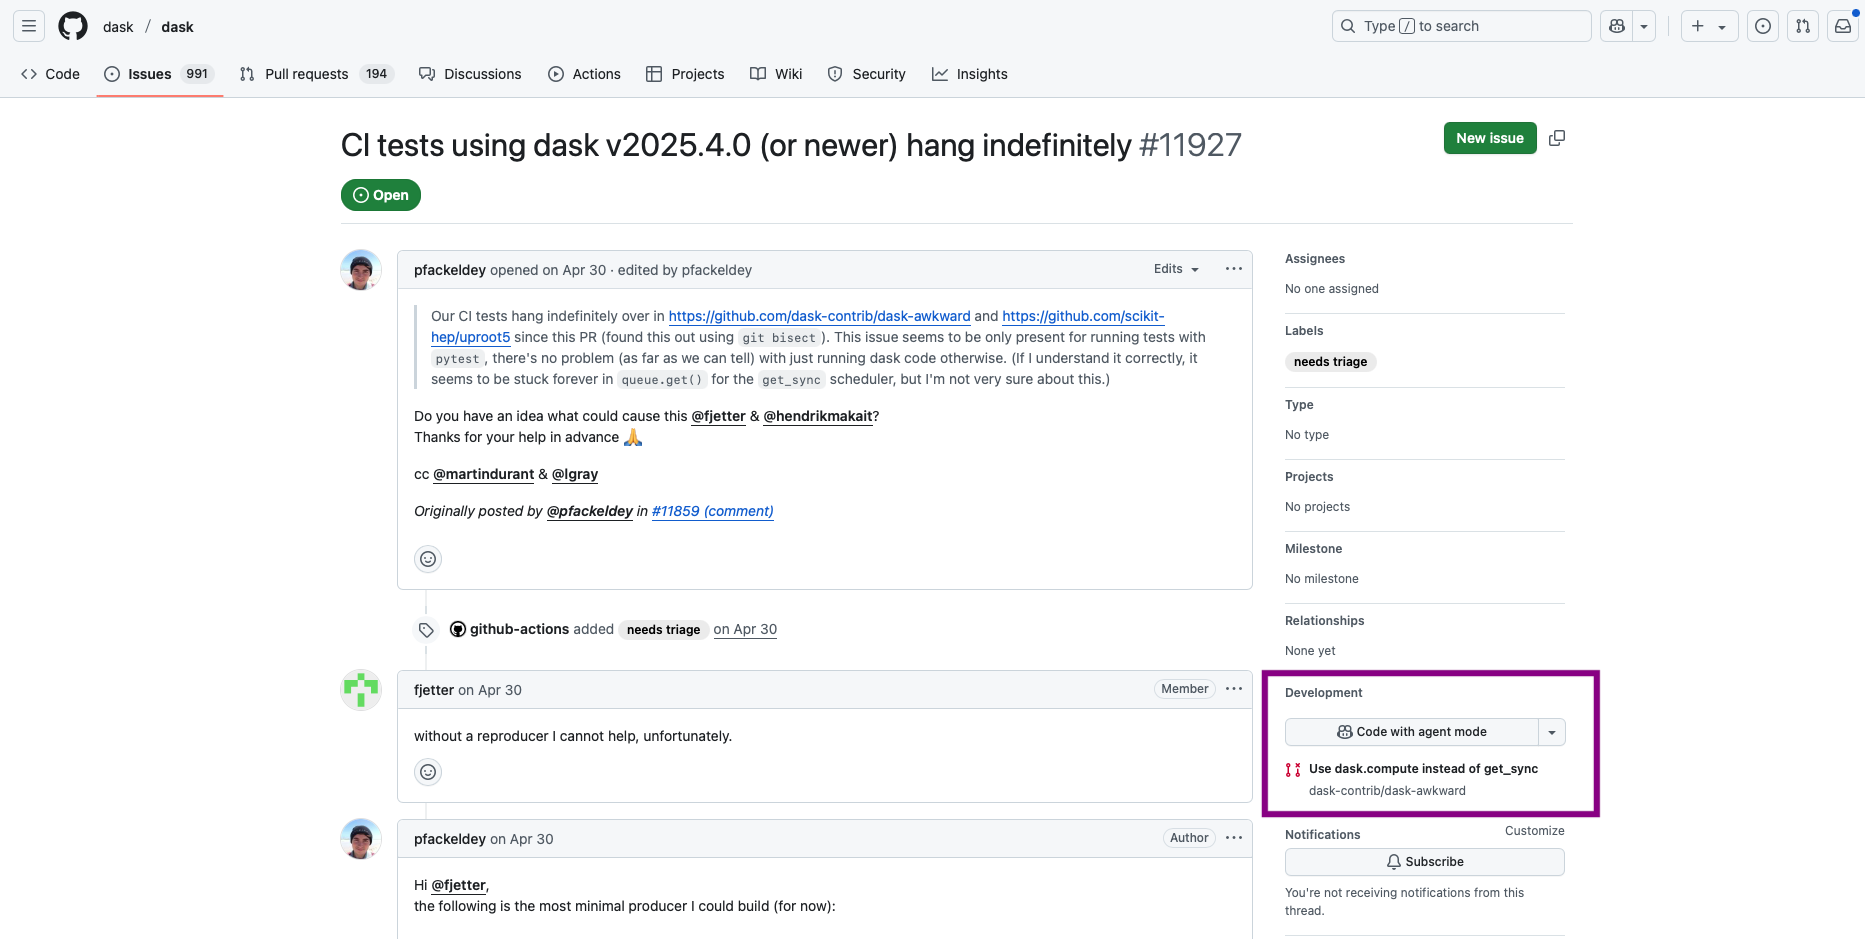
\includegraphics[width=\textwidth]{temp/dask_explainers/issue_thread.png}
  \end{subfigure}

    \bigskip
  \vspace{1ex}
  \centering
  \begin{minipage}{0.9\textwidth}
    \textbf{Figure notes:} 
    Panel~\subref{fig:dask-home} shows the \texttt{dask/dask} homepage (captured Aug 10, 12:21 PM EST).  
    The purple box links to unresolved issues (count shown); the green box links to open pull requests (count shown);  
    the orange box marks the most recent commit and its author; the red box highlights the latest release details. 
    Panel~\subref{fig:dask-issue} shows an issue thread, with the red box indicating the linked pull request. The issue was opened by user \textbf{pfackeldey} on April 30th, 2025 and received a response by \textbf{fjetter} that same day. 
  \end{minipage}

  \todo[inline]{Move to source/raw, improve title of figure}

\end{figure}
\pagebreak